% Created 2019-03-14 Thu 23:23
% Intended LaTeX compiler: pdflatex
\documentclass[presentation]{beamer}
\usepackage[utf8]{inputenc}
\usepackage[T1]{fontenc}
\usepackage{graphicx}
\usepackage{grffile}
\usepackage{longtable}
\usepackage{wrapfig}
\usepackage{rotating}
\usepackage[normalem]{ulem}
\usepackage{amsmath}
\usepackage{textcomp}
\usepackage{amssymb}
\usepackage{capt-of}
\usepackage{hyperref}
\usepackage{Schwieg}
\usepackage{natbib}
\usepackage{tikz}
\usepackage{bm}
\usepackage{minted}
\usepackage{tabularx,ragged2e,booktabs,caption}
\usetheme{Montpellier}
\author{Timothy Schwieg}
\date{\today}
\title{The Longshot bias in market data: Evidence from Counter-Strike: Global Offensive}
\hypersetup{
 pdfauthor={Timothy Schwieg},
 pdftitle={The Longshot bias in market data: Evidence from Counter-Strike: Global Offensive},
 pdfkeywords={},
 pdfsubject={},
 pdfcreator={Emacs 26.1 (Org mode 9.1.9)}, 
 pdflang={English}}
\begin{document}

\maketitle


\section{Topic}
\label{sec:org94faeea}
\begin{frame}[label={sec:orgcbb025e}]{Loot Boxes}
\begin{itemize}
\item Many video games have chosen to sell cosmetic alterations to their
games using randomization mechanisms called ``loot boxes''
\item Economic Literature tells us that there is no benefit to
randomization for risk-neutral consumers, so the benefit must come
from risk-loving consumers.
\item What aspect of these lotteries is generating the revenue for the
companies selling them?
\item How much more revenue-generating is this compared to traditional
selling mechanisms?
\end{itemize}
\end{frame}

\begin{frame}[label={sec:org65cca0a}]{Why do we care?}
\begin{itemize}
\item We are interested in discovering what drives this market to feature
randomization mechanisms.
\item Are consumers inherently more risk-loving when they play video
games?
\item Is this driven by consumers over-weighting tiny probabilities as
cumulative prospect theory suggests?
\item Are consumers weighing benefits and losses differently?
\item What is the magnitude of these gains from randomization?
\end{itemize}
\end{frame}

\section{Data}
\label{sec:org179fc23}
\begin{frame}[label={sec:orgd59b2bd}]{The Data}
\begin{itemize}
\item Contains complete market history for all items sold in the Steam
Community Market for \emph{Counter-Strike: Global Offensive}
\item Market history is specific to the hour for the last 30 days,
specific to the day for the remaining time the item has existed.
\item Contains all active buy and sell orders for each of these items as
of March 31\(^{\text{st}}\) 2018.
\item Number of active players per day and unique twitch viewers per day
\end{itemize}
\end{frame}


\begin{frame}[label={sec:orgaa7c744}]{Pictures}
\begin{center}
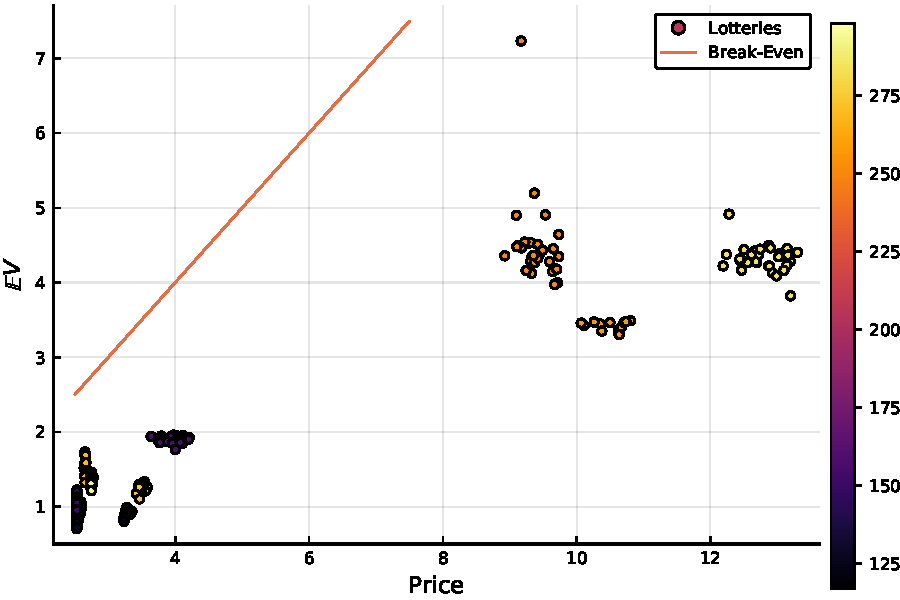
\includegraphics[width=.9\linewidth]{../Plots/BreakEvenScatter.pdf}
\end{center}
\end{frame}

\begin{frame}[label={sec:orgcdc6371}]{Does Size Matter?}
\begin{center}
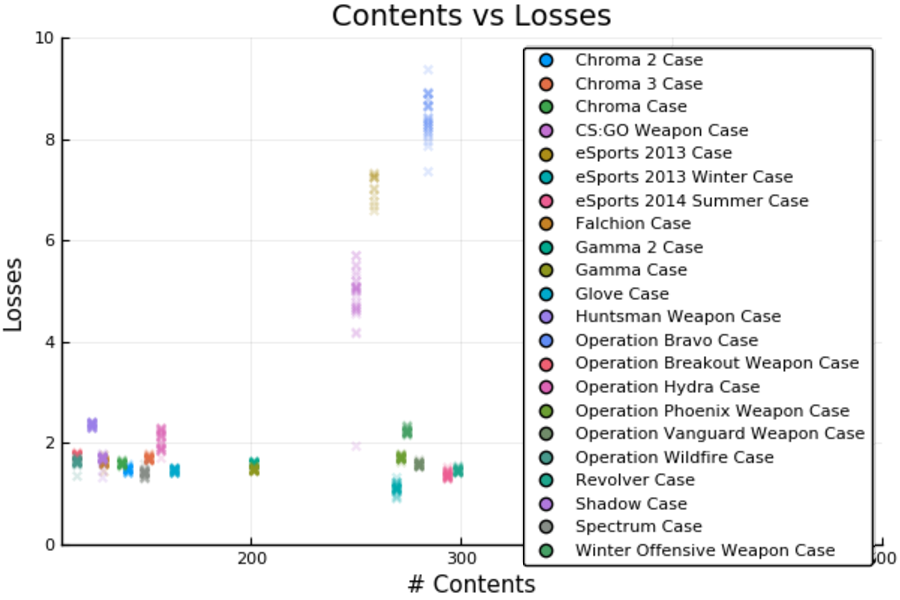
\includegraphics[width=.9\linewidth]{../Plots/LossesVSize.pdf}
\end{center}
\end{frame}

\begin{frame}[label={sec:org5dd7f37}]{Lotteries}
\begin{minipage}{\linewidth}
  \centering
  \resizebox{\columnwidth}{!}{%
  \begin{tabular}{@{}lcccccccc@{}}\toprule
    & \multicolumn{2}{c}{Values} & &\multicolumn{5}{c}{Number of Contents}\\
    \cmidrule{2-3} \cmidrule{5-9}
  Case & $\mathbb{E}[V]$ & Price &\quad& \#Blue & \#Purple & \#Pink & \#Red & \#Gold\\\midrule
Operation Wildfire  & 0.89891 & 2.5307 &\quad& 26 & 18 & 14 & 9 & 50\\
Operation Breakout  & 0.77011 & 2.5305 &\quad& 24 & 15 & 12 & 10 & 56\\
Falchion Case  & 0.95072 & 2.5323 &\quad& 27 & 24 & 11 & 9 & 59\\
Shadow Case  & 0.85299 & 2.5349 &\quad& 29 & 17 & 14 & 10 & 59\\
Huntsman Weapon Case  & 0.95531 & 3.3181 &\quad& 25 & 17 & 12 & 8 & 62\\
Spectrum Case  & 0.98146 & 2.53 &\quad& 34 & 23 & 15 & 9 & 68\\
Chroma 2 Case  & 1.0058 & 2.53 &\quad& 25 & 13 & 13 & 9 & 81\\
Chroma 3 Case  & 0.66099 & 2.53 &\quad& 30 & 19 & 11 & 10 & 81\\
Chroma Case  & 0.83215 & 2.55 &\quad& 23 & 20 & 10 & 4 & 81\\
Glove Case  & 0.84301 & 2.53 &\quad& 27 & 26 & 9 & 12 & 89\\
Operation Hydra  & 1.5465 & 4.0827 &\quad& 25 & 20 & 14 & 9 & 89\\
Gamma 2 Case  & 0.68335 & 2.53 &\quad& 31 & 22 & 13 & 7 & 128\\
Gamma Case & 0.80717 & 2.53 &\quad& 31 & 21 & 11 & 10 & 128\\\bottomrule
  \end{tabular}%
}
  
\end{minipage}
\end{frame}


\begin{frame}[label={sec:orgd5a5cfc}]{High  Content Lotteries}
\begin{minipage}{\linewidth}
  \centering
  \resizebox{\columnwidth}{!}{%
  \begin{tabular}{@{}lcccccccc@{}}\toprule
    & \multicolumn{2}{c}{Values} & &\multicolumn{5}{c}{Number of Contents}\\
    \cmidrule{2-3} \cmidrule{5-9}
  Case & $\mathbb{E}[V]$ & Price &\quad& \#Blue & \#Purple & \#Pink & \#Red & \#Gold\\\midrule
CS:GO Weapon  & 4.4611 & 9.3248 &\quad& 7 & 6 & 7 & 2 & 228\\
eSports 2013 Case  & 3.2708 & 10.354 &\quad& 8 & 13 & 7 & 2 & 228\\
eSports 2013 Winter  & 1.5687 & 2.6441 &\quad& 18 & 9 & 11 & 3 & 228\\
eSports 2014 Summer  & 1.4136 & 2.7414 &\quad& 21 & 19 & 16 & 9 & 228\\
Operation Bravo  & 4.3567 & 12.628 &\quad& 26 & 15 & 9 & 6 & 228\\
Operation Phoenix  & 0.85507 & 2.5416 &\quad& 15 & 12 & 9 & 7 & 228\\
Operation Vanguard  & 1.038 & 2.5928 &\quad& 17 & 13 & 12 & 10 & 228\\
Revolver Case  & 1.1045 & 2.53 &\quad& 24 & 25 & 12 & 9 & 228\\
Winter Offensive  & 1.299 & 3.5079 &\quad& 14 & 14 & 12 & 6 & 228\\\bottomrule
  \end{tabular}%
}
  
\end{minipage}
\end{frame}
\section{Model}
\label{sec:org52fd0ed}

\begin{frame}[label={sec:orgc7f1bcd}]{Discrete Choice - Berry (1994)}
Utility for these lotteries is quasi-linear
\begin{equation*}
  u_{ijt} = V( x_{jt}, p_{jt}; \theta ) + \xi_{jt} + \epsilon_{ij} \quad \epsilon_{ij} \sim Gumbel
\end{equation*}

Consumers choose the lottery that has the highest utility for them: 

\begin{equation*}
  \Pr( i \rightarrow j ) = \frac{\exp( V(x_{jt},p_{jt} ; \theta) + \xi_{jt})}{ \sum_{k \in \mathcal{F}}
    \exp(V(x_{jt},p_{jt}; \theta) + \xi_{kt})}
\end{equation*}

Using an outside option that is normalized so that it has zero
utility:

\begin{equation*}
  \log s_{jt} - \log s_{0t} = V(x_{jt}, p_{jt}; \theta) + \xi_{jt}
\end{equation*}
\end{frame}

\begin{frame}[label={sec:orgef47506}]{Implications}
\begin{itemize}
\item Differentiated Goods
\item Prediction based on market shares
\item Homogeneous Consumers - Is this reasonable?
\item No structure placed on \(\xi\)
\end{itemize}
\end{frame}



\begin{frame}[label={sec:org80a9964}]{Cumulative Prospect Theory}
\begin{itemize}
\item Four main components: Reference dependence, loss aversion,
diminishing sensitivity, and probability weighting

\item Diminishing sensitivity and loss aversion are summarized by the
valuation function for each content of the lottery.
\item \(x\) is not the content of the lottery, but the value of the gain or
loss of that content relative to some reference point.
\end{itemize}
\begin{align*}
  v(x) &=
  \begin{cases}
    x^\alpha \quad &x \geq 0\\
    -\lambda(-x)^\alpha \quad &x < 0
  \end{cases}\\
\end{align*}
\end{frame}

\begin{frame}[label={sec:orga96a340}]{Reference dependence and Loss Aversion}
\begin{itemize}
\item What is the proper reference point?
\item Can it be estimated?
\item How is loss aversion tied to the reference point?
\end{itemize}

\begin{center}
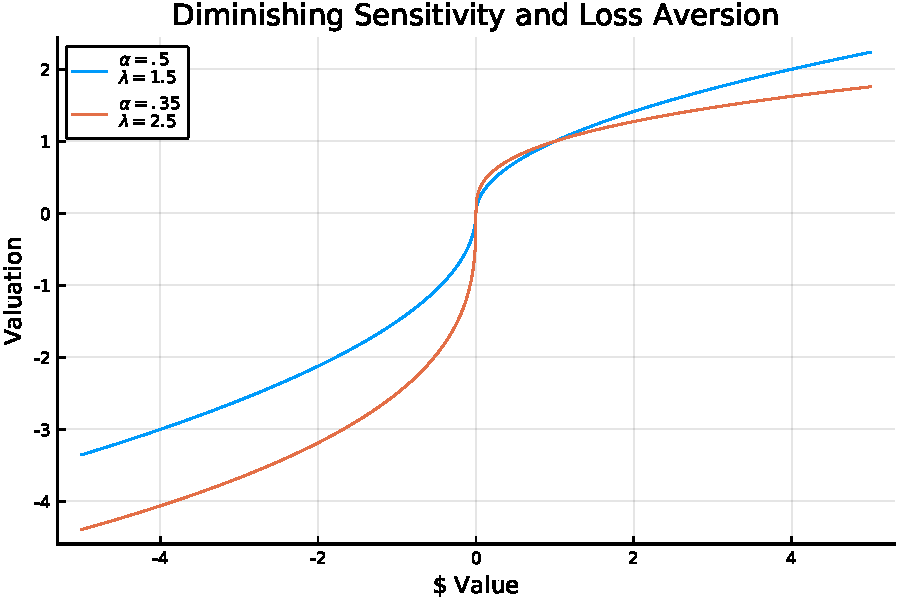
\includegraphics[width=.75\linewidth]{../Plots/ValueFunction.pdf}
\end{center}
\end{frame}

\begin{frame}[label={sec:org792a9d5}]{Probability Weighting Function}
\begin{equation*}
  w(p) = \frac{\gamma p^{\delta}}{\gamma p^{\delta} + (1-p)^{\delta}}
\end{equation*}

\begin{center}
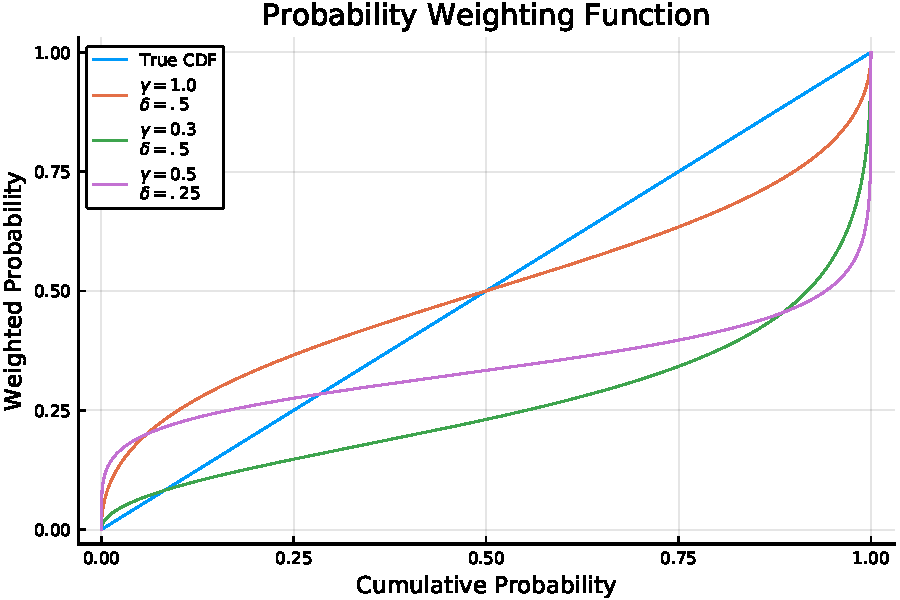
\includegraphics[width=.75\linewidth]{../Plots/WeightFun.pdf}
\end{center}
\end{frame}


\begin{frame}[label={sec:org75f7df5}]{Valuation of a Lottery}
\begin{itemize}
\item We compute the "as-if" probability taking differences of the
weighted-CDF function.
\end{itemize}
\begin{align*}
  \Pi_{s_i} &= \sum_{j=1}^{s_i} \pi_{s_j}\\
  p_i &= w( \Pi_{s_i}) - w(\Pi_{s_{i-1}})\\
  F(x_i) &= \left[  w( \Pi_{s_i}) - w(\Pi_{s_i - 1}) \right] v( x_i - R)\\
  \\
  V &= \sum_{i=1} F(x_i)\\            
\end{align*}
\end{frame}
\section{Estimation}
\label{sec:org85a7521}
\begin{frame}[label={sec:orgf234887}]{Constant Term}
\begin{itemize}
\item To normalize the utility to an outside good, need a constant term
\item There is no interpretation for this constant term.
\item Combines mis-specification of outside good, expected value of \(\xi\)
and the normalizing utility of the outside good.
\end{itemize}
\end{frame}

\begin{frame}[label={sec:orgf9116c9}]{Estimation}
\begin{itemize}
\item Price is determined by intersection of supply and demand and is
therefore endogenous
\item Instrument with the changes in daily player base from the average
number of players
\end{itemize}

\begin{align*}
  \xi_{jt} = \log s_{jt} - \log s_{0t} - \beta - V( x_{jt}, p_{jt}; \theta)
\end{align*}
Using the orthogonality of \(\xi_{jt}\) to the instruments and exogenous
parameters:
\begin{align*}
  &\min_{\bm{\xi}_{j,t}, \xi_{j,t}} \sum_{j,t}\bm{\xi}_{j,t}' \Omega \bm{\xi}_{j,t}\\
  \text{subject to: } &\xi_{j,t} = \log s_{jt} - \log s_{0t} - \beta - V( x_{jt}, p_{jt}; \theta)\\
  &\bm{\xi}_{j,t} = \xi_{j,t} \bm{Z}_{j,t}  
\end{align*}
\end{frame}

\begin{frame}[label={sec:orgc88c03f}]{Computation}
\begin{itemize}
\item Estimated using KNITRO
\item RMSE is computed both in sample and for an out-of-sample test to
determine over-fitting
\item \(\bar{R}^2\) is computed as \(1 - \frac{\mathbb{V}(\xi)}{\mathbb{V}(Y)}\)
\item J-Statistic  Critical Values:
\end{itemize}
-- Fixed Effects: 5\% 314.6784, 1\% 332.4796


-- No Fixed Effects: 5\% 337.1254, 1\% 355.5251
\end{frame}
\section{Results}
\label{sec:orgf9f9ba9}

\begin{frame}[label={sec:org7b5743c}]{Results}
\begin{minipage}{\linewidth}
  \centering
  \scalebox{0.55}{%
\begin{tabular}{@{}cccccc@{}}\toprule
  \multicolumn{3}{c}{$\exV{V}$ + Price Reference Point} & &\\
\cmidrule{1-3}
$\alpha$ & 0.56534 (2.03484) & $\lambda$ & 1.36844 (10.8477)\\
$\gamma$ & 1.0 (6.36280) & $\delta$ & 1.0 (9.47887)\\
  In Sample RMSE & 1.23649 & Out Sample RMSE & 1.4337\\
  $\bar{R}^2$ & 0.18880 & J-Statistic & 825.185\\
  \midrule
 \multicolumn{3}{c}{$\exV{V}$ + Price Reference Point and Fixed
  Effects} & &\\
\cmidrule{1-3}
$\alpha$ & 0.79549 (4.6084) & $\lambda$ & 0.60091 (9.85376)\\
$\gamma$ & 1.0 (9.79014) & $\delta$ & 1.0 (21.5814)\\
  In Sample RMSE & 1.08121 & Out Sample RMSE & 1.10642\\
  $\bar{R}^2$ & 0.51688 & J-Statistic & 558.41\\
  \midrule
\multicolumn{3}{c}{Price Reference Point} & &\\
\cmidrule{1-3}
$\alpha$ & 0.47457 (5.4068) & $\lambda$ & 0.54667 (14.56967)\\
$\gamma$ & 1.0 (10.97014) & $\delta$ & 1.0 (10.85583)\\
  In Sample RMSE & 1.52584 & Out Sample RMSE & 1.5258\\
  $\bar{R}^2$ & 0.08117 & J-Statistic & 860.261\\
  \midrule
\multicolumn{3}{c}{Price Reference Point and Fixed Effects} & &\\
\cmidrule{1-3}
$\alpha$ & 0.8215 (7.6682) & $\lambda$ & 0.3152 (7.3252)\\
$\gamma$ & 1.0 (7.6753) & $\delta$ & 1.0 (15.7306)\\
  In Sample RMSE & 1.01432 & Out Sample RMSE & 1.07900\\
  $\bar{R}^2$ & 0.54053 & J-Statistic & 351.73\\
  \midrule
\multicolumn{3}{c}{Rational - CRRA} & &\\
\cmidrule{1-3}
$\alpha$ & 0.17411 ( 6093.657) & $\beta$ & -0.32488 (0.28937)\\
  In Sample RMSE & 0.98513 & Out Sample RMSE & 1.10097\\
  $\bar{R}^2$ & 0.52163 & J-Statistic & 570.394\\\bottomrule
\end{tabular}
}
\end{minipage}
\end{frame}

\begin{frame}[label={sec:orgc133c59}]{What stories does this tell?}
\begin{itemize}
\item Rational CRRA story is one of risk aversion
\item Poor fit without fixed effects means that individuals may not be
sensitive to price changes
\item Cumulative Prospect Models do not tell a story of probability
weighting.
\item Low fit means that there is more driving this effect than a single
representative agent
\end{itemize}
\end{frame}

\begin{frame}[label={sec:org8772905}]{Where to go from here?}
\begin{itemize}
\item Belief Heterogeneity
\item Preference Heterogeneity
\item Non-parametric fit
\item Explore other alternatives for views of price
\item Larger amount of data used
\end{itemize}
\end{frame}
\end{document}